\let\negmedspace\undefined
\let\negthickspace\undefined
\documentclass[journal]{IEEEtran}
\usepackage[a5paper, margin=10mm, onecolumn]{geometry}
\usepackage{lmodern} % Ensure lmodern is loaded for pdflatex
\usepackage{tfrupee} % Include tfrupee package

\setlength{\headheight}{1cm} % Set the height of the header box
\setlength{\headsep}{0mm}     % Set the distance between the header box and the top of the text

\usepackage{gvv-book}
\usepackage{gvv}
\usepackage{cite}
\usepackage{amsmath,amssymb,amsfonts,amsthm}
\usepackage{algorithmic}
\usepackage{graphicx}
\usepackage{textcomp}
\usepackage{xcolor}
\usepackage{txfonts}
\usepackage{listings}
\usepackage{enumitem}
\usepackage{mathtools}
\usepackage{gensymb}
\usepackage{comment}
\usepackage[breaklinks=true]{hyperref}
\usepackage{tkz-euclide} 
\usepackage{listings}
% \usepackage{gvv}                                        
\def\inputGnumericTable{}                                 
\usepackage[latin1]{inputenc}                                
\usepackage{color}                                            
\usepackage{array}                                            
\usepackage{longtable}                                       
\usepackage{calc}                                             
\usepackage{multirow}                                         
\usepackage{hhline}                                           
\usepackage{ifthen}                                           
\usepackage{lscape}
\begin{document}

\bibliographystyle{IEEEtran}
\vspace{3cm}

\title{1-1.5-29}
\author{EE24BTECH11005 - Arjun Pavanje
}
% \maketitle
% \newpage
% \bigskip
{\let\newpage\relax\maketitle}
Question:\\
The coordinates of the point P dividing the line segment joining the point A(1,3) and B(4,6) in the ratio 2:1 are
\hfill (10, 2012)
\\
\solution
\begin{table}[h!]    
  \centering
  \begin{tabular}[12pt]{ |c| c|}
    \hline
    \textbf{Variable} & \textbf{Description}\\ 
    \hline
	$\vec{a}$ & $BC$ line\\
   \hline
	$\vec{b}$ & $AC$ line\\
   \hline
	$\vec{c}$ & $AB$ line, $5cm$ length\\
   \hline
	$\vec{K}$ & $a+b=5cm$\\
	\hline
	$\vec{\angle{A}}$ & $\angle{BAC}=45{\degree}$\\
	\hline

    \end{tabular}

  \caption{Variables Used}
  \label{tab1-1.5-29}
\end{table}\\
If $P$ divides $AB$ in the ratio $k:1$,


\begin{align} 
P=\frac{kB+A}{k+1} 
\end{align}\\
\begin{align}
	P = \frac{\myvec{
4k+1 \\
6k+3
}}{k+1} 
\end{align}\\
here, $k = 2$, so putting the $k$ we get
\begin{align}
P = 
\myvec{
3\\
5
}
\end{align}
The coordinates of the required point $P$ are
\begin{align}
\myvec{
3\\
5
}
\end{align}
\begin{figure}[h!]
   \centering
   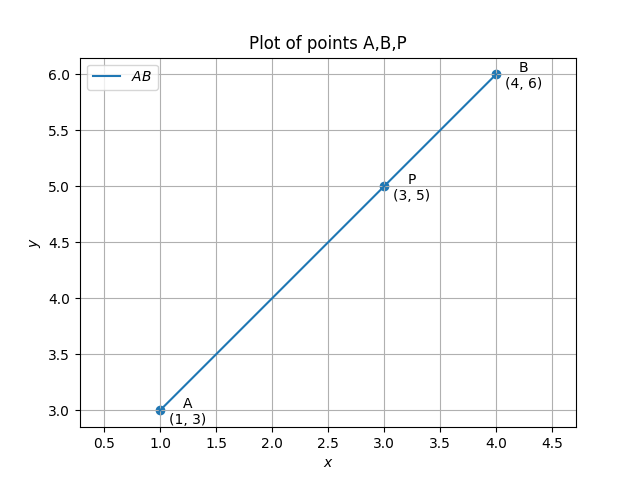
\includegraphics[width=0.7\linewidth]{figs/Figure_1.png}
   \caption{Plot of the points A,B,P}
   \label{stemplot}
\end{figure}
\end{document}
